\documentclass[11pt,a4paper]{article}

\usepackage[margin=2.2cm]{geometry}
\usepackage{amsmath,amssymb,booktabs,array,longtable,xcolor,enumitem,hyperref,listings,tikz}
\usetikzlibrary{arrows.meta,positioning,fit,calc,decorations.pathreplacing}
\usepackage[T1]{fontenc}
\usepackage{lmodern}

\hypersetup{colorlinks=true,linkcolor=blue!55!black,urlcolor=blue!55!black}
\setlist{nosep,leftmargin=*}
\lstset{
  basicstyle=\ttfamily\small,
  columns=fullflexible,
  frame=single,
  breaklines=true,
  showstringspaces=false,
  keywordstyle=\color{blue!55!black},
  commentstyle=\color{green!40!black}
}

\newcommand{\hpose}[2]{h_{#1}\!\left(b^{#2}\right)}

\title{MR-BSP Entropy Scope and Implementation Map\\
\large Issues 11--15: historical audit, simulation comparison, and definitive Visual-SLAM logic}
\author{ANPLOS / MR-BSP working note}
\date{9 September 2026}

\begin{document}
\maketitle

\section{Conclusion}

The Visual-SLAM implementation does not use a true joint-covariance entropy.
Its planning score is a separable team score: the sum of the focused marginal
entropy scores around the final positions of Robot A and Robot B.  Therefore,
if a realized-entropy column is intended to be the execution-time counterpart
of a particular robot's Step-1 prediction, it must again contain two terms,
both calculated from that robot's execution posterior:
\[
  H_{\mathrm{real}}^A
  = \hpose{A}{A,\mathrm{exec}}+\hpose{B}{A,\mathrm{exec}},
  \qquad
  H_{\mathrm{real}}^B
  = \hpose{A}{B,\mathrm{exec}}+\hpose{B}{B,\mathrm{exec}}.
\]

The current rollout does not do this.  Its ``Robot A realized entropy'' is only
Robot A's final-pose marginal, and its ``Robot B realized entropy'' is only
Robot B's final-pose marginal.  The dashboard then adds those two values, even
though they came from two different local beliefs.  That arithmetic sum can be
reported as a decentralized self-uncertainty performance statistic, but it is
not the realized value of either robot's Step-1 objective.

\section{What the publication defines}

The publication defines one cooperative objective, evaluated from the local
belief of the robot performing the calculation:
\[
  J(b_k^r,a_{k+}).
\]
The superscript $r$ identifies the \emph{belief perspective}; it does not turn
$J$ into a cost concerning only robot $r$.  The state, observations, and
actions are joint, and all robots use the same cooperative reward function.
The Visual-SLAM terminal reward is written as
\[
  \rho_L(b_{k+L}^r)
  =-\beta H(b_{k+L}^r)
   -(1-\beta)\,
    \mathbb E\!\left[
      d(g^r,\xi^r_{k+L-1})+d(g^{r'},\xi^{r'}_{k+L-1})
    \right].
\]

Thus, the distance component explicitly includes both robots.  The entropy
component is described only as $H(b^r)$, ``the entropy of the belief.''  The
current manuscript does \emph{not} explicitly state that this is implemented
as the sum of two final-position marginal entropy scores.  That specialization
must be stated in the new resubmission if it remains the experimental metric.

The manuscript also assumes that the actions of other robots are available to
robot $r$, while their observations may be only partially shared.  This
distinction determines which factors may legitimately appear in a robot's
execution posterior.

\section{The implemented focused entropy}

For a final pose $X_i$ with $6\times6$ pose covariance $\Sigma_i$, the code
keeps the translational $3\times3$ block and calculates
\[
  h_i
  =\frac{1}{2}\log\det\!\left(\Sigma_i^{\mathrm{pos}}\right).
\]
The Gaussian additive constant is omitted.  Rotation uncertainty is also
omitted.  This is therefore an entropy-like focused uncertainty score, with
the same action ordering as the corresponding Gaussian positional entropy
when the dimensionality is fixed.

For each candidate joint action, the Step-1 planner selects the last pose of
each robot and sums the two scores:
\[
  H_{\mathrm{pred}}^r(a)
  = \hpose{A}{r,\mathrm{pred}}(a)
   +\hpose{B}{r,\mathrm{pred}}(a).
\]
Both covariances in this equation come from the same predicted posterior belief
$b_{\mathrm{pred}}^r$ maintained by the planning robot.

This is \emph{not} the entropy of a full joint covariance.  A true joint
entropy would require the block covariance
\[
  \Sigma_{AB}
  =\begin{bmatrix}
      \Sigma_A & \Sigma_{AB}^{\mathrm{cross}}\\
      (\Sigma_{AB}^{\mathrm{cross}})^\mathsf T & \Sigma_B
    \end{bmatrix}
\]
and would depend on the cross-covariance between the endpoint poses.  The
implemented score deliberately ignores that cross-covariance and adds the two
marginal scores instead.

\section{What the current rollout calculates}

For each robot $r$, the current execution evaluator:
\begin{enumerate}
  \item loads the saved candidate posterior graph for the action selected by
        robot $r$;
  \item samples or loads a physical ground-truth realization;
  \item generates image measurements by projecting known landmarks through
        the realized trajectory;
  \item replaces candidate-path vision factors for the robot being evaluated;
  \item optimizes the resulting factor graph;
  \item extracts only that robot's final-pose marginal covariance; and
  \item converts only that covariance to focused entropy.
\end{enumerate}

Ground truth is not itself an uncertainty distribution.  It supplies the
physical poses and landmarks used to generate measurements.  The uncertainty
comes from the posterior covariance after estimation:
\[
  \begin{aligned}
  \text{ground truth}
  &\longrightarrow \text{simulated measurements}
  \longrightarrow \text{posterior factor graph}\\
  &\longrightarrow \text{marginal covariance}
  \longrightarrow \text{focused entropy}.
  \end{aligned}
\]

The two current dashboard columns are therefore
\[
  E_A^{\mathrm{current}}=\hpose{A}{A,\mathrm{exec}},
  \qquad
  E_B^{\mathrm{current}}=\hpose{B}{B,\mathrm{exec}}.
\]
The displayed sum is
\[
  E_{\mathrm{self\mbox{-}sum}}^{\mathrm{current}}
  =\hpose{A}{A,\mathrm{exec}}+\hpose{B}{B,\mathrm{exec}}.
\]
It combines two self-marginals obtained from two different local beliefs.  It
is a meaningful external team statistic if labelled that way, but it does not
equal $H_{\mathrm{real}}^A$ or $H_{\mathrm{real}}^B$.

\section{Issue 12: historical Table 3 and execution-code audit}

The historical implementation gives an unambiguous answer about the scope of
the Visual-SLAM objective.  Table 3 did \emph{not} report a realized
post-execution entropy.  Its ``Objective Values ($J$)'' column reported the
Step-1 planning-time hybrid objective of the chosen candidate joint action,
computed from the reference robot's belief.  The reference robot was Robot A
in the table-generation path.

For a candidate joint action $a$, the historical code calculated
\begin{align}
 H_{\mathrm{pred}}^A(a)
 &=h_A\!\left(b_{\mathrm{pred}}^A(a)\right)
   +h_B\!\left(b_{\mathrm{pred}}^A(a)\right), \\
 \widehat J\!\left(b_k^A,a\right)
 &=-0.95\,H_{\mathrm{pred}}^A(a)
   -0.05\bigl(\ell_A(a)+\ell_B(a)\bigr).
 \label{eq:historical-table3-j}
\end{align}
Here, both endpoint covariances are extracted from the \emph{same} predicted
posterior constructed from Robot A's available belief.  Each endpoint score is
\begin{equation}
 h_i\!\left(b_{\mathrm{pred}}^A(a)\right)
 =\frac{1}{2}\log\det
   \Sigma^{A,\mathrm{pred}}_{i,\mathrm{final},xyz}(a),
 \qquad i\in\{A,B\}.
\end{equation}
The path-length mode used for these results was \texttt{last}, so
$\ell_A+\ell_B$ is the sum of the final motion segment for each robot.  The
stored \texttt{hybrid\_obj} is the maximum of
\eqref{eq:historical-table3-j} across candidate joint actions.  The
table-generation code then selected the appropriate communication iteration
for Baseline II, R-EnforceAC, or Baseline I and reported the mean and standard
deviation across runs.

This historical metric is therefore best described as:
\begin{quote}
the sum of Robot A's marginal focused uncertainty about Robot A's final
predicted pose and Robot A's marginal focused uncertainty about Robot B's
final predicted pose, both conditioned on Robot A's current information.
\end{quote}
It is not a one-robot entropy, not a true joint entropy, not the sum of two
independently computed self-entropies, and not an oracle calculation.  Only
Baseline I has full shared data; Baseline II and R-EnforceAC use Robot A's
belief at their respective communication states.

\subsection{Numerical reproduction of the Table 3 value 11.35}

For seed 0 at the Baseline-II communication state, historical saved data for
the selected candidate contain
\[
 h_A=-6.0180656,\qquad h_B=-6.1756823,\qquad
 \ell_A+\ell_B=4.7059834.
\]
Consequently,
\begin{align*}
 H_{\mathrm{pred}}^A
 &=-6.0180656-6.1756823=-12.1937479,\\
 \widehat J
 &=-0.95(-12.1937479)-0.05(4.7059834)\\
 &=11.3487613\approx 11.35,
\end{align*}
which exactly reproduces the Baseline-II entry in Table 3.  At full
communication, the corresponding saved value is $13.4300764$, reproducing
the reported Baseline-I value $13.43$.

\subsection{Why Table 3 is not evidence of realized entropy}

The results pipeline copied
\texttt{results[Robot\_A][step\_1][hybrid\_obj]} into the per-iteration
summary.  Step-2 and Step-3 sampled objectives were used to test whether the
Step-1 action remained preferred, but they did not replace the reported
$J$-value.  Table 3 therefore measures a predicted planning score for the
selected action, not uncertainty recomputed after execution.

The historical file also contains a separate function named
\texttt{get\_entropies\_post\_exec}.  Its intended scope is nevertheless
clear: it constructs one post-execution belief from Robot A's available data
and one from Robot B's available data, requests both final-pose covariances in
each belief, and intends to return
\[
 H_{\mathrm{post}}^A
 =h_A(b_{\mathrm{post}}^A)+h_B(b_{\mathrm{post}}^A),
 \qquad
 H_{\mathrm{post}}^B
 =h_A(b_{\mathrm{post}}^B)+h_B(b_{\mathrm{post}}^B).
\]
Thus, the historical design agrees with the two-endpoint, one-belief-at-a-time
scope adopted for the Issue-11-fixed experiments.  It does not add Robot A's
self-entropy from $b^A$ to Robot B's self-entropy from $b^B$.

There is an implementation caveat: in the audited historical revision,
\texttt{get\_entropies\_post\_exec} called
\texttt{cov\_mat\_to\_focused\_entropy} with one argument although the helper
required the pose symbol and covariance matrix.  This legacy post-execution
path was separate from Table 3 and was not used to generate its $J$ column.
The defect affects whether that legacy function could execute successfully;
it does not make its intended two-endpoint scope ambiguous.

\section{Exact factor scope: legacy versus corrected execution logic}

Consider Robot A evaluating execution after a planning history ending at
$A20,B20$.  Suppose Robot B communicated visual observations only through
$B12$, while its observations from $B13$ through $B20$ remained private.
Write $\mathcal F_{i,[u:v]}$ for all motion and visual factors of robot $i$
over an interval, $\mathcal M_i^{\mathrm{exec}}$ for execution motion factors,
and $\mathcal V_i^{\mathrm{exec}}$ for execution vision factors.

\subsection{What is always valid in Robot A's local execution posterior}

Robot A may condition on:
\begin{enumerate}
  \item its complete local history $\mathcal F_{A,[0:20]}$, including factors
        involving landmarks that were never shared with Robot B;
  \item the communicated part $\mathcal F_{B,[0:12]}$ of Robot B's history;
  \item both robots' actually executed motion factors
        $\mathcal M_A^{\mathrm{exec}}$ and
        $\mathcal M_B^{\mathrm{exec}}$, because the experiment assumes that
        the executed actions are known; and
  \item all new camera measurements acquired locally by Robot A,
        $\mathcal V_A^{\mathrm{exec}}$.
\end{enumerate}
Robot B's private historical vision factors from $B13$ through $B20$ must
remain absent.  Robot B's execution vision factors may enter Robot A's belief
only if those measurements were explicitly communicated.

Accordingly, the corrected Robot-A factor set is
\begin{align}
 \mathcal F_{\mathrm{exec}}^{A,\mathrm{correct}}
 ={}&\mathcal F_{A,[0:20]}
 \cup\mathcal F_{B,[0:12]}^{\mathrm{shared}}
 \cup\mathcal M_A^{\mathrm{exec}}
 \cup\mathcal M_B^{\mathrm{exec}}
 \cup\mathcal V_A^{\mathrm{exec}} .
 \label{eq:correct-a-factor-set}
\end{align}
Unless communication occurs after execution,
\[
 \mathcal F_{B,[13:20]}^{\mathrm{vision}}\not\subset
 \mathcal F_{\mathrm{exec}}^{A,\mathrm{correct}},
 \qquad
 \mathcal V_B^{\mathrm{exec}}\not\subset
 \mathcal F_{\mathrm{exec}}^{A,\mathrm{correct}}.
\]
After optimizing this one Robot-A-local graph, the corrected score is
\[
 H_{\mathrm{real}}^A
 =h_A\!\left(b_{\mathrm{exec}}^A\right)
  +h_B\!\left(b_{\mathrm{exec}}^A\right).
\]
The Robot-B calculation is symmetric.

Ground truth or a simulated physical trajectory may be used offline to
generate a noisy measurement.  That operation does not automatically make
the measurement available to every robot.  A projection from Robot B's
realized pose becomes a factor in Robot A's posterior only when the modeled
communication protocol delivers that observation to A.

\subsection{What the legacy post-execution function intended}

The legacy \texttt{get\_entropies\_post\_exec} construction appended the
complete execution interval of both robots to each local post-execution
belief.  For Robot A, its intended factor set was effectively
\begin{align}
 \mathcal F_{\mathrm{exec}}^{A,\mathrm{legacy}}
 ={}&\mathcal F_{A,[0:20]}
 \cup\mathcal F_{B,[0:12]}^{\mathrm{shared}}
 \cup\mathcal M_A^{\mathrm{exec}}
 \cup\mathcal V_A^{\mathrm{exec}} \nonumber\\
 &{}\cup\mathcal M_B^{\mathrm{exec}}
 \cup\mathcal V_B^{\mathrm{exec}} .
 \label{eq:legacy-a-factor-set}
\end{align}
Thus, the description \emph{all of A's data, B's shared prefix, and both
robots' complete execution segments} correctly describes the legacy
function's intended graph.  The gap $B13$--$B20$ remained absent, but B's
execution vision factors reappeared after $B20$.  This implicitly assumes that
B's new execution observations become available to A even though its older
private observations do not.

That assumption is not valid for the corrected robot-local metric unless
post-execution communication is explicitly part of the protocol.  Moreover,
the legacy function had the call-signature defect described above and did not
produce Table 3.

\section{Which logic corresponds to which experiment}

\begin{longtable}{>{\raggedright\arraybackslash}p{0.19\textwidth}
                  >{\raggedright\arraybackslash}p{0.25\textwidth}
                  >{\raggedright\arraybackslash}p{0.46\textwidth}}
\toprule
Artifact or experiment & Quantity and belief scope & Factor and entropy logic \\
\midrule
\endfirsthead
\toprule
Artifact or experiment & Quantity and belief scope & Factor and entropy logic \\
\midrule
\endhead
\bottomrule
\endlastfoot
Published Visual-SLAM Table 3 &
Step-1 projected hybrid objective $\widehat J$ from Robot A's belief &
Sums the focused marginal entropies of A's and B's final
\emph{predicted} poses inside Robot A's candidate posterior, then combines
that sum with both final path segments using weights $0.95$ and $0.05$.
It is not realized entropy and does not use the legacy post-execution
function. \\

Legacy post-execution path &
Intended post-execution entropy, one two-endpoint result per robot-local belief &
The \texttt{verify\_against\_bsln} and
\texttt{get\_entropies\_post\_exec} path uses the legacy factor scope in
\eqref{eq:legacy-a-factor-set}, including the
peer's complete execution vision interval.  The path was unused for Table 3
and contained a call-signature defect. \\

Moshe/Tanmoy search-and-rescue simulations &
Whole binary-grid entropy inside each agent's local grid belief &
Robot locations are known exactly.  Planning marginalizes over transition,
cell-state, and observation outcomes; execution samples a transition and a
noisy cell observation.  Bayesian cell updates replace pose-graph inference:
there are no pose covariances, odometry factors, projection factors, or
landmark variables. \\

Dashboard Experiment 22 &
Original 30-seed sequential-evidence operating point &
Original realized columns contain only each robot's own final-pose marginal.
Their displayed sum combines self-marginals from two different beliefs; it is
not either robot's two-endpoint realized objective. \\

Dashboard Experiment 23 &
Original early instantaneous operating point &
Uses the same original one-endpoint-per-perspective realized-entropy scope as
Experiment 22. \\

Dashboard Experiment 24 &
Original late instantaneous operating point &
Uses the same original one-endpoint-per-perspective realized-entropy scope as
Experiment 22. \\

Dashboard Experiment 25:
Definitive metric, execution-only landmarks included ($\chi=1$) &
Primary corrected variant of Experiment 22 &
Uses \eqref{eq:correct-a-factor-set} separately for each belief perspective;
adds both final-pose marginal focused entropies inside that one posterior;
adds only the evaluating robot's execution vision; and admits landmarks that
were invisible throughout both prior trajectories and are first triangulated
from that robot's local execution images. \\

Dashboard Experiment 26:
Definitive metric, execution-only landmarks excluded ($\chi=0$) &
Known-landmarks-only ablation of Experiment 25 &
Uses the identical Experiment-22 geometry, seeds, decisions, acceptance rows,
and two-endpoint robot-local calculation as Experiment 25, but a landmark
absent from the complete prior cannot enter the execution graph. \\

Dashboard Experiment 27:
Experiment 24 (Issue 11 fixed) &
Earlier corrected copy retained for provenance &
Uses the corrected two-endpoint robot-local scope on the late instantaneous
operating point; it predates the explicit $\chi=1$ versus $\chi=0$ pair. \\
\end{longtable}

Experiments 25 and 26 preserve Experiment 22's planning decisions and
acceptance mechanism exactly.  Their only mutual difference is $\chi$.
Experiment 27 remains the earlier late-operating-point corrected copy.  None
of these turns realized entropy into the full hybrid $J$ reported by the
historical Table 3: no path-length term is added to the realized entropy
columns.

\section{Step-1 projected entropy versus realized entropy}

They are not, in general, the same quantity.  Two separate distinctions are
important: metric scope and prediction versus realization.

\subsection{Original Experiments 22--24: different scope}

In the original experiment implementation, robot $r$'s Step-1 projected
entropy is
\[
  H_{\mathrm{pred}}^r(a_r^*)
  =\hpose{A}{r,\mathrm{pred}}(a_r^*)
   +\hpose{B}{r,\mathrm{pred}}(a_r^*),
\]
whereas its reported realized entropy is only
\[
  E_{r,\mathrm{old}}^{\mathrm{real}}
  =\hpose{r}{r,\mathrm{exec}}.
\]
The old values therefore cannot be compared directly: the Step-1 value has
two endpoint terms and the realized value has one.

\subsection{Issue-11-fixed experiments: matching scope, different stage}

The fixed realized metric uses the same two-endpoint scope:
\[
  H_{\mathrm{real}}^r
  =\hpose{A}{r,\mathrm{exec}}+\hpose{B}{r,\mathrm{exec}}.
\]
Even after this correction, $H_{\mathrm{pred}}^r$ and
$H_{\mathrm{real}}^r$ are not expected to be numerically identical.

Step 1 constructs a deterministic predicted posterior from the robot's
pre-execution belief, nominal candidate motion, and maximum-likelihood
geometric observations generated from predicted poses and current landmark
estimates.  It produces one projected entropy value for each candidate action.

The realized calculation instead uses the action components actually executed,
a sampled physical trajectory and landmark realization, noisy camera
measurements generated from that realization, and only the information
available to the evaluating robot.  Repeating this process gives a Monte Carlo
distribution summarized by a mean and standard deviation.

The comparison is therefore
\[
  \underbrace{H_{\mathrm{pred}}^r(a_r^*)}_{
    \substack{\text{predicted before execution}\\
              \text{nominal/MLE future observations}}}
  \quad\text{versus}\quad
  \underbrace{\mathbb E\!\left[H_{\mathrm{real}}^r\right]}_{
    \substack{\text{estimated after simulated execution}\\
              \text{actual action pair and noisy observations}}}.
\]

At an action-inconsistent row, the difference is even more fundamental.  The
physical action pair contains A's component of A's decision and B's component
of B's decision, so it need not equal either robot's complete Step-1 proposed
joint action.

The two values would coincide only under restrictive conditions: both robots
execute exactly the joint candidate assumed in Step 1; the realized visible
factor set equals the predicted factor set; the realized measurements equal
their nominal maximum-likelihood values; both calculations condition on the
same information; and nonlinear optimization produces the same linearization.
In a linear-Gaussian model with a fixed factor structure, measurement values
do not change the covariance, making equality more plausible.  Visual SLAM is
nonlinear and its visibility and linearization can change, so equality is not
guaranteed even at an action-consistent row.

Consequently, the scientifically meaningful quantity is the prediction error
or calibration gap
\[
  \Delta H^r
  =\mathbb E\!\left[H_{\mathrm{real}}^r\right]
   -H_{\mathrm{pred}}^r(a_r^*),
\]
reported only after both terms use the same two-endpoint scope.  A zero value
means the predicted uncertainty was calibrated to the realized mean; it is not
an identity imposed by the algorithm.

\section{How to construct a valid execution posterior}

For each robot $r$, construct $b_{\mathrm{exec}}^r$ from the information that
is actually in that robot's history.  The construction should start from the
robot's real local belief immediately before execution, not from a Step-1
candidate posterior containing hypothetical future observations.

For Robot A, the valid construction is:
\begin{enumerate}
  \item Preserve Robot A's complete local motion and visual history.
  \item Preserve only the portion of Robot B's past visual observations that
        was actually communicated to A.
  \item Preserve or append Robot B's motion chain where its actions are known,
        in accordance with the paper's action-availability assumption.
  \item Append the motion factors corresponding to the actions actually
        executed by A and B.
  \item Add every new visual observation genuinely acquired by A during
        execution, including A-local landmark observations that were never
        shared with B.
  \item Add new observations acquired by B only if those observations were
        actually communicated to A by the evaluation time.
  \item Optimize once, extract the marginal positional covariances of both
        final poses, and sum their focused entropy scores.
\end{enumerate}

Robot B's execution posterior is constructed symmetrically.

In the fixed implementation, saved pose values from the selected candidate may
be used as an \emph{initial guess} for nonlinear optimization of the newly
appended trajectory.  This is not an information factor: no candidate visual
factor is copied, and the posterior information matrix is still defined only
by the valid local prior, the executed motion factors, the evaluating robot's
available execution observations, and the existing weak numerical landmark
priors.  This distinction matters because pure odometric initialization can
leave a large-residual visual-SLAM problem outside the convergence basin even
when the factor graph itself is valid.

For numerical integrity, a measurement realization is never silently replaced
merely because the default GTSAM marginalization rejects an ill-conditioned
linear system.  The evaluator first retries the \emph{same} realization from
the alternative candidate-based initial guess.  If both nonlinear attempts
remain ill-conditioned, it computes the local Laplace covariance from that
same graph and linearization using a symmetric Moore--Penrose pseudoinverse of
$J^{\mathsf T}J$.  The dashboard records how many realizations used each
fallback.  A new noisy realization is drawn only if all three calculations
fail.  The final fixed datasets require zero such rejected realizations.

\subsection{The missing B12--B20 observations}

Suppose A knows B's motion history through B20 but has received B's camera
observations only through B12.  Then B13--B20 pose variables and motion factors
may legitimately exist in A's belief, while B13--B20 private vision factors do
not.  The missing observations must remain absent.  Their absence correctly
causes A's uncertainty about B to grow through the motion chain.

It would be invalid to generate B13--B20 image factors from ground truth merely
to fill the gap.  It would be equally invalid to begin inserting B's private
execution image factors after B20 unless those measurements were communicated.
The fact that ground truth makes such projections possible for an offline
evaluator does not make those factors part of Robot A's information history.

\section{What happens when the robots choose different actions}

When Step 1 is inconsistent, Robot A's chosen action index and Robot B's chosen
action index may refer to different proposed joint actions.  The physical
execution is not either complete proposal.  Each robot executes its own
component, producing a mixed realized joint action:
\[
  a_{\mathrm{exec}}
  =\left(a_A^{\text{chosen by A}},
          a_B^{\text{chosen by B}}\right).
\]

Because the paper assumes that selected actions are communicated after
planning and in parallel with execution, a post-execution belief may condition
on this actual action pair.  If the metric were instead evaluated before the
peer action became known, the evaluator would have to marginalize over the
unknown peer action rather than silently substitute either robot's prediction.

\section{Why the current saved posterior cannot simply be reused}

The Step-1 candidate graph contains predicted motion and maximum-likelihood
geometric factors for both robots' candidate paths.  The current rollout
removes and regenerates candidate vision factors only for the pose prefix being
evaluated.  Hypothetical peer future factors can therefore remain in the graph
and can indirectly change the evaluated robot's covariance through shared
landmarks.

Consequently, the correct two-endpoint calculation is not merely:
\begin{quote}
``Ask the current rollout graph for the other final covariance and add it.''
\end{quote}
The evaluator must begin from the pre-execution local graph, strip all
hypothetical future measurements, add the actual motion pair, and add only the
observations available to the relevant robot.

\section{Three distinct metrics that must not be conflated}

\begin{longtable}{>{\raggedright\arraybackslash}p{0.24\textwidth}
                  >{\raggedright\arraybackslash}p{0.34\textwidth}
                  >{\raggedright\arraybackslash}p{0.32\textwidth}}
\toprule
Metric & Definition & Interpretation \\
\midrule
\endfirsthead
\toprule
Metric & Definition & Interpretation \\
\midrule
\endhead
\bottomrule
\endlastfoot
Robot-A-perspective realized team score &
$\hpose{A}{A,\mathrm{exec}}+\hpose{B}{A,\mathrm{exec}}$ &
Realized counterpart of Robot A's Step-1 predicted entropy. \\

Robot-B-perspective realized team score &
$\hpose{A}{B,\mathrm{exec}}+\hpose{B}{B,\mathrm{exec}}$ &
Realized counterpart of Robot B's Step-1 predicted entropy. \\

Decentralized self-entropy sum &
$\hpose{A}{A,\mathrm{exec}}+\hpose{B}{B,\mathrm{exec}}$ &
External system statistic formed from each robot's uncertainty about itself;
not one robot's $J$. \\

Centralized full-data score &
$h_A(b^{\mathrm{central}})+h_B(b^{\mathrm{central}})$ &
Oracle or Baseline-I-style benchmark using all observations from both robots;
not an R-VerifyAC robot-local posterior. \\

True joint entropy &
$\tfrac12\log\det\Sigma_{AB}$, up to the Gaussian constant &
Uses the full endpoint block covariance including cross-correlation; not
computed by the current planner. \\
\end{longtable}

\section{Definitive realized-entropy convention agreed with Moshe}

The final decision is to evaluate execution strictly from the information
available to the robot whose result is being reported.  There is no oracle
posterior and no cross-belief sum.  Let $s$ be the last communicated pose index
and let $+$ denote the end of execution (for example, $A_{30}$ and $B_{30}$).
Write
\begin{itemize}
  \item $\mathcal M_i^{0:+}$ for all motion factors of robot $i$ from its
        initial pose through the end of execution;
  \item $\mathcal V_i^{0:+}$ for all actual vision factors acquired by robot
        $i$ over the same interval; and
  \item $\mathcal V_i^{0:s,\mathrm{shared}}$ for the prefix of robot $i$'s
        vision factors that was communicated to the peer.
\end{itemize}

Under the paper's assumption that executed actions are known, both robots know
both complete motion chains.  Under partial observation sharing, each robot
knows its own complete vision history but only the communicated prefix of the
peer's vision history.  Therefore Robot A's execution graph is
\begin{equation}
 \boxed{
 \mathcal F_A^{\mathrm{exec}}(\chi)
 =\mathcal M_A^{0:+}
  \cup\mathcal V_A^{0:+}(\chi)
  \cup\mathcal M_B^{0:+}
  \cup\mathcal V_B^{0:s,\mathrm{shared}} }
 \label{eq:definitive-factor-a}
\end{equation}
and Robot B's mirror computation is
\begin{equation}
 \boxed{
 \mathcal F_B^{\mathrm{exec}}(\chi)
 =\mathcal M_B^{0:+}
  \cup\mathcal V_B^{0:+}(\chi)
  \cup\mathcal M_A^{0:+}
  \cup\mathcal V_A^{0:s,\mathrm{shared}} .}
 \label{eq:definitive-factor-b}
\end{equation}
In particular,
\[
 \mathcal V_B^{s+1:+}\not\subset\mathcal F_A^{\mathrm{exec}},
 \qquad
 \mathcal V_A^{s+1:+}\not\subset\mathcal F_B^{\mathrm{exec}}.
\]
Shared-landmark variables and their communicated projection factors may connect
the two motion chains inside either local graph.  What matters is factor
provenance: the factor must have been measured locally or received through the
communication protocol.

\subsection{Optional inclusion of landmarks first discovered during execution}

The switch $\chi\in\{0,1\}$ controls whether a robot includes landmarks that
were absent from every pre-execution belief but were first detected by its own
camera during execution:
\[
 \mathcal V_i^{0:+}(\chi)=
 \begin{cases}
  \mathcal V_{i,\mathrm{known}}^{0:+}, & \chi=0,\\
  \mathcal V_{i,\mathrm{known}}^{0:+}
   \cup\mathcal V_{i,\mathrm{new}}^{\mathrm{exec}}, & \chi=1.
 \end{cases}
\]
The primary real-execution interpretation is $\chi=1$, because these are real
measurements acquired by the evaluating robot.  The $\chi=0$ setting is a
controlled known-landmarks-only ablation.  The switch is applied symmetrically:
A may add newly detected A-side landmarks only to $b_A^{\mathrm{exec}}$, and B
may add newly detected B-side landmarks only to $b_B^{\mathrm{exec}}$, unless
the corresponding measurements are later communicated.

\subsection{Why the missing peer vision factors cannot be manufactured}

Robot A cannot construct a realized observation from $B_{18}$ or $B_{22}$
merely because its estimate predicts that a landmark should be visible:
\begin{enumerate}
  \item Projecting Robot A's maximum-likelihood estimates of the peer pose and
        landmark would create a \emph{predicted pseudo-measurement}.  That is a
        legitimate Step-1 planning operation, not an execution measurement.
  \item Projecting the hidden simulated ground-truth peer pose and landmark
        would create a physically plausible Robot-B measurement, but making it
        available to Robot A would leak oracle information across the stated
        communication boundary.
  \item In a real experiment, the measurement could originate only from Robot
        B's sensor.  By assumption, Robot A has no access to that sensor stream
        unless B communicates the observation.
\end{enumerate}
Mixing ground-truth-generated local factors with estimate-generated peer
pseudo-factors and calling both ``realized observations'' would therefore mix
planning and execution semantics.

Ground truth is used only by the simulator's generative side:
\[
 (X_i^{\mathrm{GT}},L_j^{\mathrm{GT}})
 \xrightarrow{\text{pinhole projection + sensor noise}} z_{ij}.
\]
The estimator receives $z_{ij}$ and the noise model, never
$X_i^{\mathrm{GT}}$ or $L_j^{\mathrm{GT}}$.  Consequently, only the robot that
acquired $z_{ij}$ may insert its projection factor before communication.

\subsection{One optimization and two focused marginals per robot}

Each robot optimizes its own complete execution graph exactly once:
\[
 \widehat\Theta_r
 =\arg\min_{\Theta}
   \sum_{f\in\mathcal F_r^{\mathrm{exec}}(\chi)}
   \lVert e_f(\Theta)\rVert^2_{\Omega_f},
 \qquad r\in\{A,B\}.
\]
From the optimized local posterior, it extracts the translational marginal
covariances of \emph{both} final robot poses:
\[
 \Sigma_{A+}^{,r}=\operatorname{MargCov}_{b_r^{\mathrm{exec}}}(A_+)_{xyz},
 \qquad
 \Sigma_{B+}^{,r}=\operatorname{MargCov}_{b_r^{\mathrm{exec}}}(B_+)_{xyz}.
\]
The two focused entropy terms and their sum are
\begin{align}
 h_A^r&=\tfrac12\log\det\Sigma_{A+}^{,r},
 &h_B^r&=\tfrac12\log\det\Sigma_{B+}^{,r},\\
 H_{\mathrm{real}}^r&=h_A^r+h_B^r,
 &r&\in\{A,B\}.
 \label{eq:definitive-realized-score}
\end{align}
Thus $H_{\mathrm{real}}^A$ and $H_{\mathrm{real}}^B$ will generally differ.
Typically A knows its own final pose better than B knows A's final pose, and B
knows its own final pose better than A knows B's final pose.  This difference
is expected evidence of decentralized information, not an inconsistency in the
metric.

For naming precision, $H_{\mathrm{real}}^r$ is the raw realized entropy score.
The corresponding entropy reward is $-H_{\mathrm{real}}^r$.  If the paper's
full hybrid objective is reported, then
\[
 J_{\mathrm{real}}^r
 =-\beta H_{\mathrm{real}}^r
  -(1-\beta)(\ell_A+\ell_B).
\]
Calling the positive entropy sum itself ``$J$'' is acceptable only if the table
explicitly declares that $J$ denotes the entropy component rather than the
signed hybrid reward.

\clearpage
\section{System-level illustrations}

The following diagrams use the structure of the handwritten sketch: two robot
trajectories, a shared-history boundary, an execution interval, the sensing
updates, and the inference output.  Solid arrows denote motion evolution;
dashed colored links denote sensing information.  The diagrams deliberately
separate information used to create a robot's posterior from hidden simulator
ground truth used only to generate measurements.

\subsection{Historical Visual-SLAM implementation}

\begin{figure}[!ht]
\centering
\resizebox{\textwidth}{!}{%
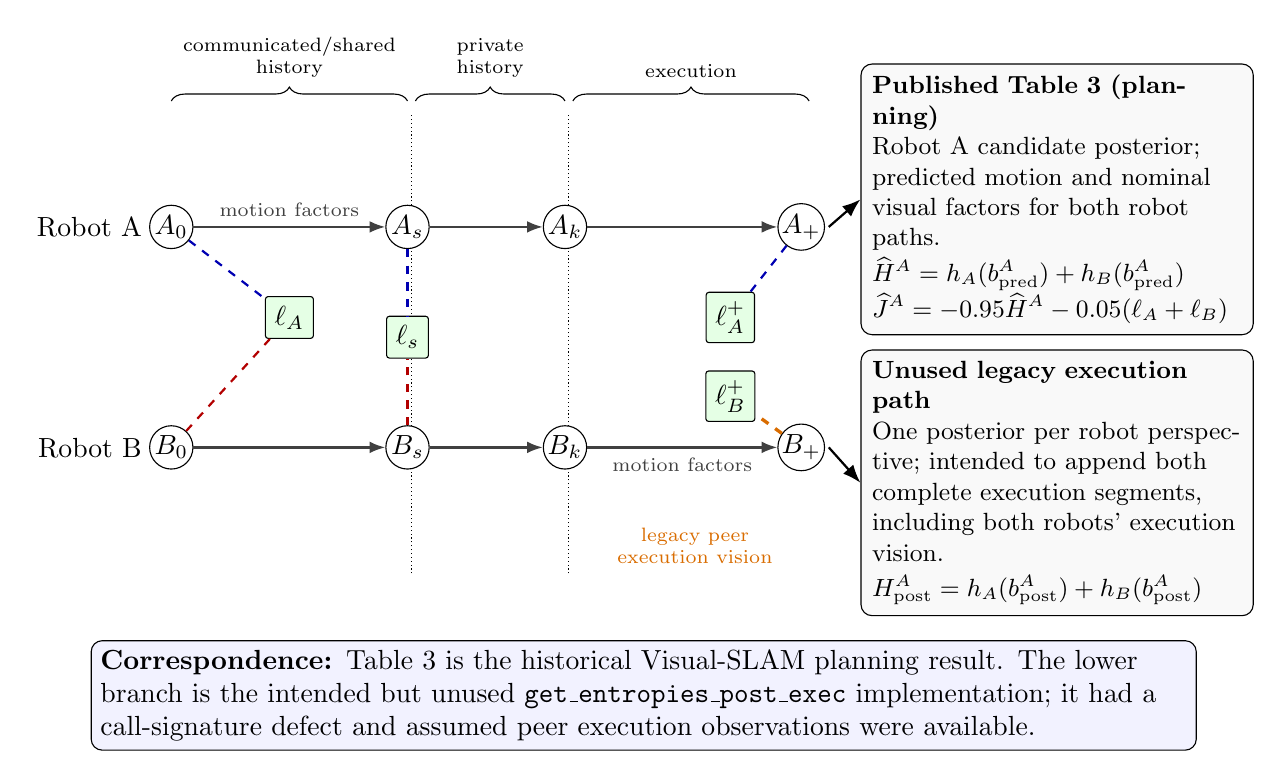
\begin{tikzpicture}[
  pose/.style={circle,draw,minimum size=5.5mm,inner sep=0pt,fill=white},
  landmark/.style={rectangle,draw,rounded corners=1pt,minimum size=5mm,fill=green!10},
  motion/.style={-{Latex[length=2mm]},thick,black!75},
  visionA/.style={dashed,thick,blue!70!black},
  visionB/.style={dashed,thick,red!70!black},
  legacy/.style={dashed,very thick,orange!85!black},
  box/.style={draw,rounded corners,align=left,fill=gray!5,inner sep=4pt,text width=4.7cm,font=\small},
  note/.style={align=center,font=\small}
]
  \draw[decorate,decoration={brace,amplitude=5pt}] (0,5.8)--(3.0,5.8)
    node[midway,above=5pt,note,font=\scriptsize]{communicated/shared\\history};
  \draw[decorate,decoration={brace,amplitude=5pt}] (3.1,5.8)--(5.0,5.8)
    node[midway,above=5pt,note,font=\scriptsize]{private\\history};
  \draw[decorate,decoration={brace,amplitude=5pt}] (5.1,5.8)--(8.1,5.8)
    node[midway,above=5pt,note,font=\scriptsize]{execution};
  \draw[densely dotted] (3.05,-0.2)--(3.05,5.65);
  \draw[densely dotted] (5.05,-0.2)--(5.05,5.65);

  \node[left] at (-0.25,4.2) {Robot A};
  \node[pose] (A0) at (0,4.2) {$A_0$};
  \node[pose] (As) at (3,4.2) {$A_s$};
  \node[pose] (Ak) at (5,4.2) {$A_k$};
  \node[pose] (Ae) at (8,4.2) {$A_+$};
  \draw[motion] (A0)--node[above,font=\scriptsize]{motion factors}(As);
  \draw[motion] (As)--(Ak);
  \draw[motion] (Ak)--(Ae);

  \node[left] at (-0.25,1.4) {Robot B};
  \node[pose] (B0) at (0,1.4) {$B_0$};
  \node[pose] (Bs) at (3,1.4) {$B_s$};
  \node[pose] (Bk) at (5,1.4) {$B_k$};
  \node[pose] (Be) at (8,1.4) {$B_+$};
  \draw[motion] (B0)--(Bs);
  \draw[motion] (Bs)--(Bk);
  \draw[motion] (Bk)--node[below,font=\scriptsize]{motion factors}(Be);

  \node[landmark] (La) at (1.5,3.05) {$\ell_A$};
  \node[landmark] (Ls) at (3.0,2.8) {$\ell_s$};
  \node[landmark] (Lea) at (7.1,3.05) {$\ell_A^+$};
  \node[landmark] (Leb) at (7.1,2.05) {$\ell_B^+$};
  \draw[visionA] (A0)--(La); \draw[visionA] (As)--(Ls);
  \draw[visionB] (B0)--(La); \draw[visionB] (Bs)--(Ls);
  \draw[visionA] (Ae)--(Lea);
  \draw[legacy] (Be)--(Leb);
  \node[font=\scriptsize,orange!85!black,align=center] at (6.65,0.15)
    {legacy peer\\execution vision};

  \node[box] (table3) at (11.25,4.55) {
    \textbf{Published Table 3 (planning)}\\
    Robot A candidate posterior; predicted motion and nominal visual factors
    for both robot paths.\\[2pt]
    $\widehat H^A=h_A(b^A_{\rm pred})+h_B(b^A_{\rm pred})$\\
    $\widehat J^A=-0.95\widehat H^A-0.05(\ell_A+\ell_B)$};
  \node[box] (post) at (11.25,0.95) {
    \textbf{Unused legacy execution path}\\
    One posterior per robot perspective; intended to append both complete
    execution segments, including both robots' execution vision.\\[2pt]
    $H^A_{\rm post}=h_A(b^A_{\rm post})+h_B(b^A_{\rm post})$};
  \draw[-{Latex},thick] (8.35,4.2)--(table3.west);
  \draw[-{Latex},thick] (8.35,1.4)--(post.west);

  \node[draw,rounded corners,fill=blue!5,align=left,text width=13.8cm]
    at (6.0,-1.75) {\textbf{Correspondence:} Table 3 is the historical
    Visual-SLAM planning result.  The lower branch is the intended but unused
    \texttt{get\_entropies\_post\_exec} implementation; it had a call-signature
    defect and assumed peer execution observations were available.};
\end{tikzpicture}%
}
\caption{Historical Visual-SLAM planning and intended legacy execution logic.
Blue and red dashed links are Robot-A and Robot-B vision factors; orange marks
the peer-execution vision admitted by the legacy post-execution construction.}
\label{fig:historical-visual-slam-flow}
\end{figure}

\clearpage

\subsection{Moshe/Tanmoy search-and-rescue simulations}

The search-and-rescue experiment is structurally simpler than Visual SLAM.
The hidden state is a binary target-occupancy grid.  Robot locations are
treated as exactly known, so there is no pose posterior and no distinction
between robot-specific pose entropy terms.  Each agent evaluates the entropy
of its own current belief over the \emph{entire grid}:
\[
 H(b^r)=-\sum_i\sum_{x_i\in\{0,1\}}
 b^r(x_i)\log b^r(x_i).
\]

\begin{figure}[!ht]
\centering
\resizebox{0.98\textwidth}{!}{%
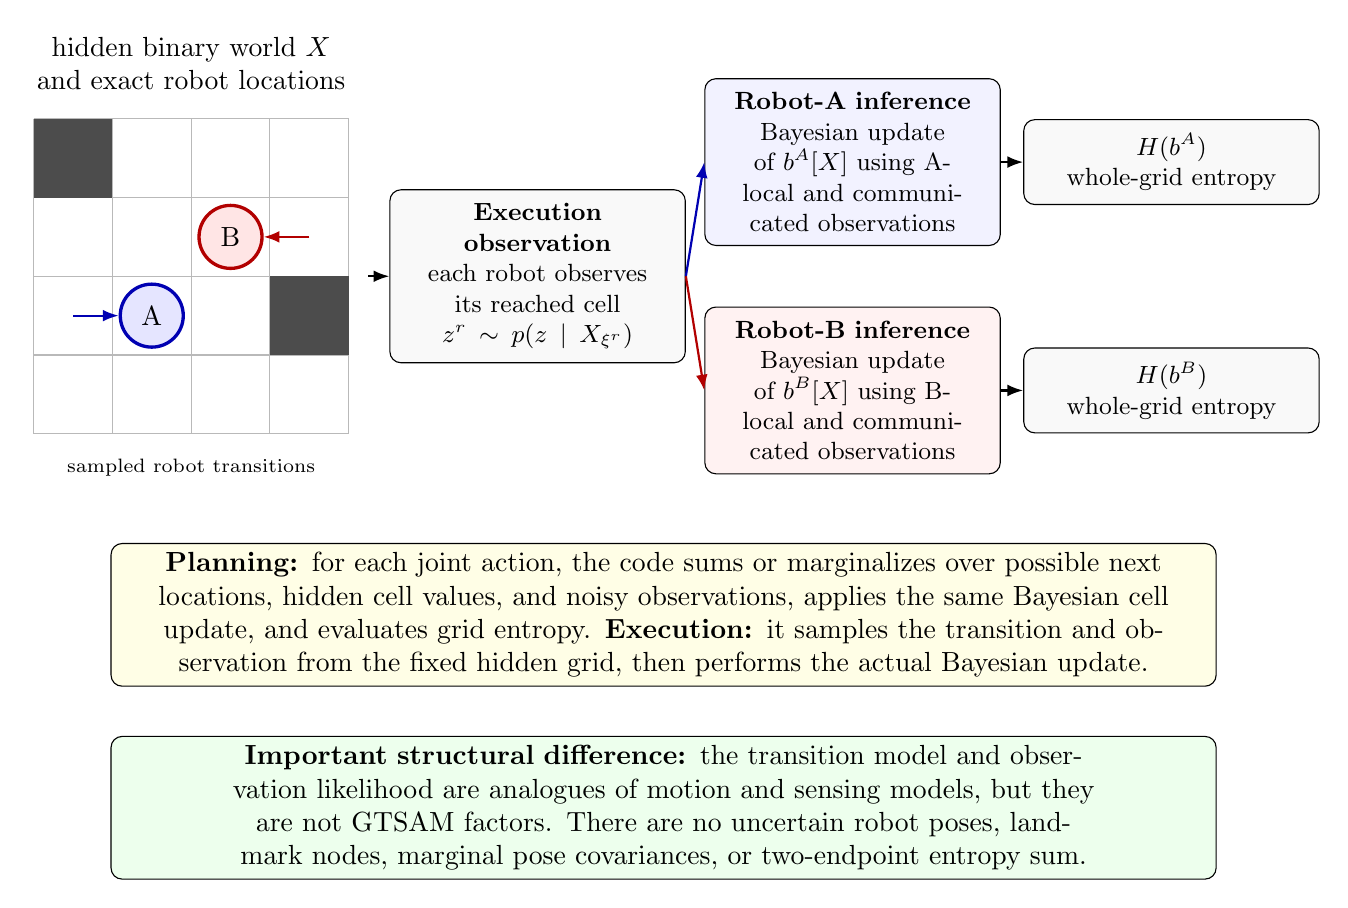
\begin{tikzpicture}[
  flow/.style={-{Latex[length=2mm]},thick},
  box/.style={draw,rounded corners,align=center,fill=gray!5,inner sep=5pt,text width=3.4cm,font=\small},
  robotA/.style={circle,draw=blue!70!black,very thick,fill=blue!10,minimum size=8mm},
  robotB/.style={circle,draw=red!70!black,very thick,fill=red!10,minimum size=8mm}
]
  \begin{scope}[shift={(0,0)}]
    \foreach \x in {0,...,4} {\draw[gray!55] (\x,0)--(\x,4);}
    \foreach \y in {0,...,4} {\draw[gray!55] (0,\y)--(4,\y);}
    \fill[black!70] (0,3) rectangle (1,4);
    \fill[black!70] (3,1) rectangle (4,2);
    \node[robotA] (RA) at (1.5,1.5) {A};
    \node[robotB] (RB) at (2.5,2.5) {B};
    \draw[flow,blue!70!black] (0.5,1.5)--(RA);
    \draw[flow,red!70!black] (3.5,2.5)--(RB);
    \node[above,align=center] at (2,4.25) {hidden binary world $X$\\and exact robot locations};
    \node[below,align=center,font=\scriptsize] at (2,-0.2)
      {sampled robot transitions};
  \end{scope}

  \node[box] (obs) at (6.4,2.0) {\textbf{Execution observation}\\
    each robot observes its reached cell\\
    $z^r\sim p(z\mid X_{\xi^r})$};
  \draw[flow] (4.25,2.0)--(obs.west);

  \node[box,fill=blue!5] (ba) at (10.4,3.45) {\textbf{Robot-A inference}\\
    Bayesian update of $b^A[X]$ using A-local and communicated observations};
  \node[box,fill=red!5] (bb) at (10.4,0.55) {\textbf{Robot-B inference}\\
    Bayesian update of $b^B[X]$ using B-local and communicated observations};
  \draw[flow,blue!70!black] (obs.east)--(ba.west);
  \draw[flow,red!70!black] (obs.east)--(bb.west);

  \node[box] (ha) at (14.45,3.45) {$H(b^A)$\\whole-grid entropy};
  \node[box] (hb) at (14.45,0.55) {$H(b^B)$\\whole-grid entropy};
  \draw[flow] (ba)--(ha); \draw[flow] (bb)--(hb);

  \node[draw,rounded corners,fill=yellow!10,align=center,text width=13.8cm]
    at (8.0,-2.30) {\textbf{Planning:} for each joint action, the code sums or
    marginalizes over possible next locations, hidden cell values, and noisy
    observations, applies the same Bayesian cell update, and evaluates grid
    entropy.  \textbf{Execution:} it samples the transition and observation
    from the fixed hidden grid, then performs the actual Bayesian update.};
  \node[draw,rounded corners,fill=green!7,align=center,text width=13.8cm]
    at (8.0,-4.75) {\textbf{Important structural difference:} the transition
    model and observation likelihood are analogues of motion and sensing
    models, but they are not GTSAM factors.  There are no uncertain robot poses,
    landmark nodes, marginal pose covariances, or two-endpoint entropy sum.};
\end{tikzpicture}%
}
\caption{Moshe/Tanmoy search-and-rescue simulation, verified against the Julia
simulation and the paper's simulation section.  Both robots reason about the
same type of team state---the entire target grid---from different local beliefs.}
\label{fig:grid-simulation-flow}
\end{figure}

\clearpage

\subsection{Definitive current Visual-SLAM convention}

\begin{figure}[!ht]
\centering
\resizebox{\textwidth}{!}{%
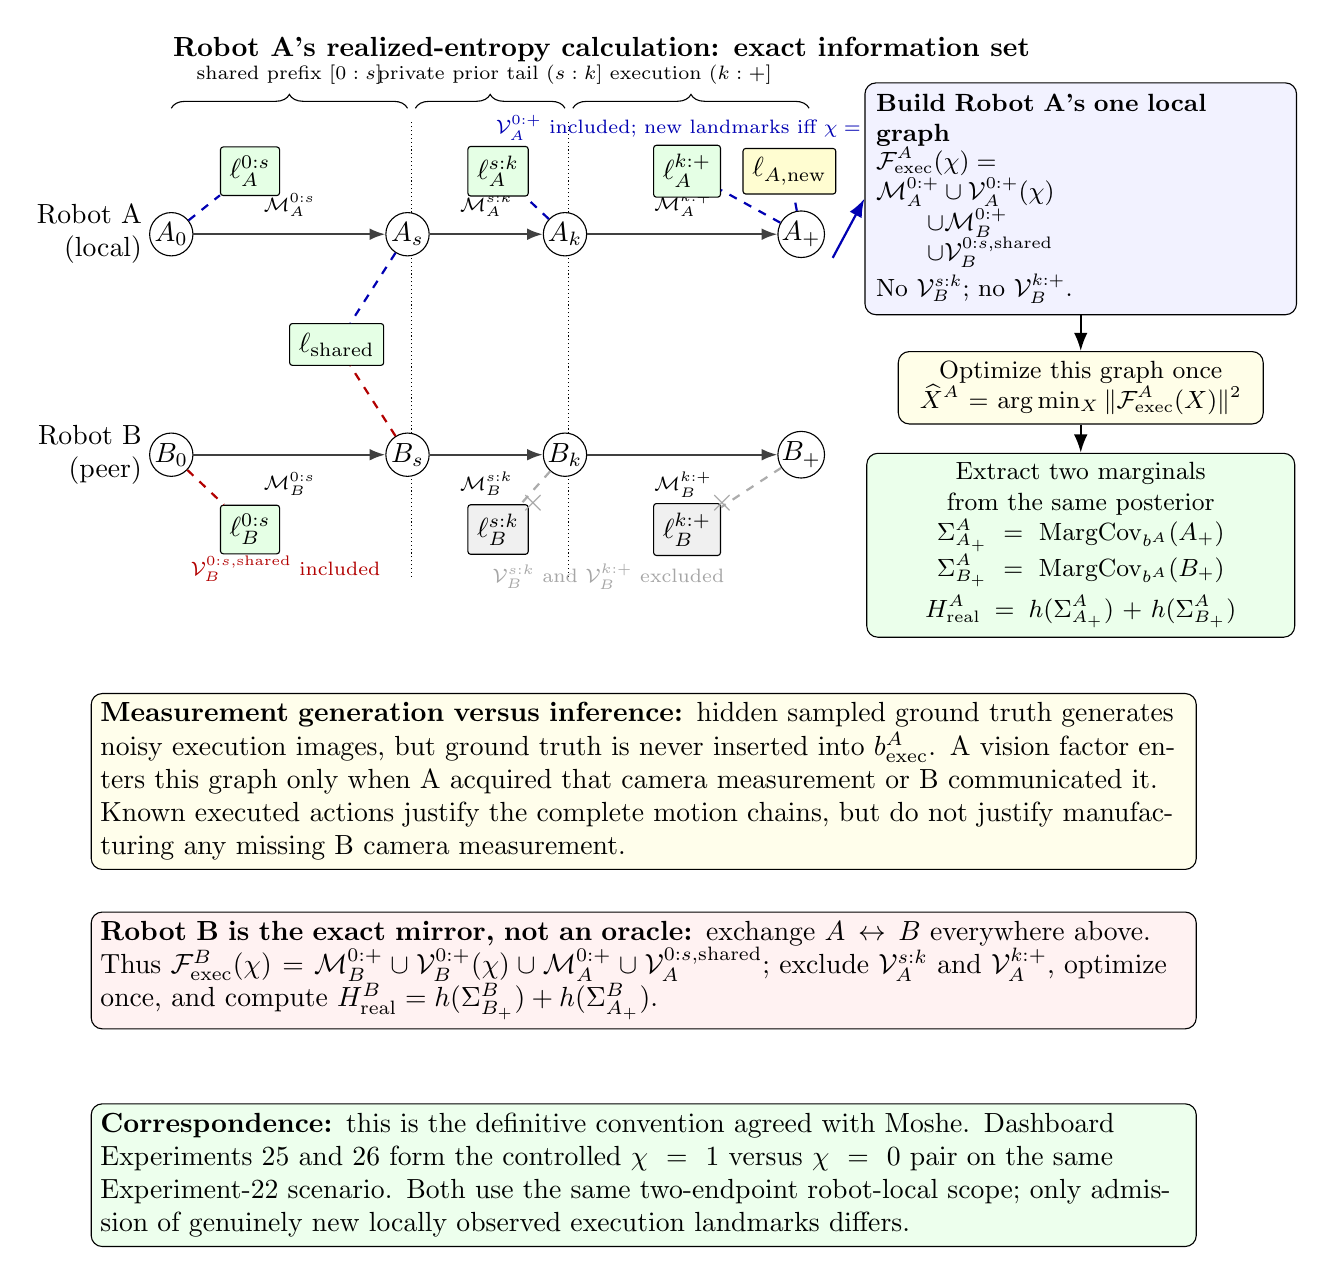
\begin{tikzpicture}[
  pose/.style={circle,draw,minimum size=5.5mm,inner sep=0pt,fill=white},
  landmark/.style={rectangle,draw,rounded corners=1pt,minimum size=5mm,fill=green!10},
  motion/.style={-{Latex[length=2mm]},thick,black!75},
  visionA/.style={dashed,thick,blue!70!black},
  visionB/.style={dashed,thick,red!70!black},
  excluded/.style={dashed,thick,gray!65},
  box/.style={draw,rounded corners,align=left,fill=gray!5,inner sep=4pt,text width=4.9cm,font=\small},
  note/.style={align=center,font=\small}
]
  \node[anchor=west,font=\bfseries] at (-0.1,6.55)
    {Robot A's realized-entropy calculation: exact information set};
  \draw[decorate,decoration={brace,amplitude=5pt}] (0,5.8)--(3.0,5.8)
    node[midway,above=5pt,note,font=\scriptsize]{shared prefix $[0:s]$};
  \draw[decorate,decoration={brace,amplitude=5pt}] (3.1,5.8)--(5.0,5.8)
    node[midway,above=5pt,note,font=\scriptsize]{private prior tail $(s:k]$};
  \draw[decorate,decoration={brace,amplitude=5pt}] (5.1,5.8)--(8.1,5.8)
    node[midway,above=5pt,note,font=\scriptsize]{execution $(k:+]$};
  \draw[densely dotted] (3.05,-0.15)--(3.05,5.65);
  \draw[densely dotted] (5.05,-0.15)--(5.05,5.65);

  \node[left,align=right] at (-0.25,4.2) {Robot A\\(local)};
  \node[pose] (A0) at (0,4.2) {$A_0$};
  \node[pose] (As) at (3,4.2) {$A_s$};
  \node[pose] (Ak) at (5,4.2) {$A_k$};
  \node[pose] (Ae) at (8,4.2) {$A_+$};
  \draw[motion] (A0)--(As); \draw[motion] (As)--(Ak); \draw[motion] (Ak)--(Ae);
  \node[font=\scriptsize,above] at (1.5,4.3) {$\mathcal M_A^{0:s}$};
  \node[font=\scriptsize,above] at (4.0,4.3) {$\mathcal M_A^{s:k}$};
  \node[font=\scriptsize,above] at (6.5,4.3) {$\mathcal M_A^{k:+}$};

  \node[left,align=right] at (-0.25,1.4) {Robot B\\(peer)};
  \node[pose] (B0) at (0,1.4) {$B_0$};
  \node[pose] (Bs) at (3,1.4) {$B_s$};
  \node[pose] (Bk) at (5,1.4) {$B_k$};
  \node[pose] (Be) at (8,1.4) {$B_+$};
  \draw[motion] (B0)--(Bs); \draw[motion] (Bs)--(Bk); \draw[motion] (Bk)--(Be);
  \node[font=\scriptsize,below] at (1.5,1.3) {$\mathcal M_B^{0:s}$};
  \node[font=\scriptsize,below] at (4.0,1.3) {$\mathcal M_B^{s:k}$};
  \node[font=\scriptsize,below] at (6.5,1.3) {$\mathcal M_B^{k:+}$};

  \node[landmark] (Ls) at (2.1,2.8) {$\ell_{\rm shared}$};
  \node[landmark] (La0) at (1.0,5.0) {$\ell_A^{0:s}$};
  \node[landmark] (Lap) at (4.15,5.0) {$\ell_A^{s:k}$};
  \node[landmark] (Lae) at (6.55,5.0) {$\ell_A^{k:+}$};
  \node[landmark,fill=yellow!18] (Lan) at (7.85,5.0) {$\ell_{A,\rm new}$};
  \node[landmark] (Lb0) at (1.0,0.45) {$\ell_B^{0:s}$};
  \node[landmark,fill=gray!12] (Lbp) at (4.15,0.45) {$\ell_B^{s:k}$};
  \node[landmark,fill=gray!12] (Lbe) at (6.55,0.45) {$\ell_B^{k:+}$};
  \draw[visionA] (A0)--(La0); \draw[visionA] (Ak)--(Lap);
  \draw[visionA] (Ae)--(Lae); \draw[visionA] (Ae)--(Lan);
  \draw[visionA] (As)--(Ls); \draw[visionB] (Bs)--(Ls);
  \draw[visionB] (B0)--(Lb0);
  \draw[excluded] (Bk)--(Lbp); \draw[excluded] (Be)--(Lbe);
  \node[font=\scriptsize,blue!70!black,align=center] at (6.55,5.55)
    {$\mathcal V_A^{0:+}$ included; new landmarks iff $\chi=1$};
  \node[font=\scriptsize,red!70!black] at (1.45,-0.05)
    {$\mathcal V_B^{0:s,\rm shared}$ included};
  \node[font=\scriptsize,gray!70,align=center] at (5.55,-0.15)
    {$\mathcal V_B^{s:k}$ and $\mathcal V_B^{k:+}$ excluded};
  \node[font=\large,gray!70] at (4.6,0.78) {$\times$};
  \node[font=\large,gray!70] at (7.0,0.78) {$\times$};

  \node[box,fill=blue!5,text width=5.2cm] (graph) at (11.55,4.65) {
    \textbf{Build Robot A's one local graph}\\[-1pt]
    $\mathcal F^A_{\rm exec}(\chi)=$\\
    $\mathcal M_A^{0:+}\cup\mathcal V_A^{0:+}(\chi)$\\
    $\qquad\cup\mathcal M_B^{0:+}$\\
    $\qquad\cup\mathcal V_B^{0:s,\rm shared}$\\[2pt]
    No $\mathcal V_B^{s:k}$; no $\mathcal V_B^{k:+}$.};
  \node[draw,rounded corners,fill=yellow!9,align=center,font=\small,
        text width=4.4cm] (opt) at (11.55,2.25) {
    Optimize this graph once\\
    $\widehat X^A=\arg\min_X\|\mathcal F^A_{\rm exec}(X)\|^2$};
  \node[draw,rounded corners,fill=green!8,align=center,font=\small,
        text width=5.2cm] (marg) at (11.55,0.25) {
    Extract two marginals from the same posterior\\
    $\Sigma^A_{A_+}=\operatorname{MargCov}_{b^A}(A_+)$\\
    $\Sigma^A_{B_+}=\operatorname{MargCov}_{b^A}(B_+)$\\[2pt]
    $H^A_{\rm real}=h(\Sigma^A_{A_+})+h(\Sigma^A_{B_+})$};
  \draw[-{Latex},thick,blue!70!black] (8.4,3.9)--(graph.west);
  \draw[-{Latex},thick] (graph)--(opt);
  \draw[-{Latex},thick] (opt)--(marg);

  \node[draw,rounded corners,fill=yellow!8,align=left,text width=13.8cm]
    at (6.0,-2.75) {\textbf{Measurement generation versus inference:}
    hidden sampled ground truth generates noisy execution images, but ground
    truth is never inserted into $b^A_{\rm exec}$.  A vision factor enters this
    graph only when A acquired that camera measurement or B communicated it.
    Known executed actions justify the complete motion chains, but do not
    justify manufacturing any missing B camera measurement.};
  \node[draw,rounded corners,fill=red!5,align=left,text width=13.8cm]
    at (6.0,-5.15) {\textbf{Robot B is the exact mirror, not an oracle:}
    exchange $A\leftrightarrow B$ everywhere above.  Thus
    $\mathcal F^B_{\rm exec}(\chi)=
    \mathcal M_B^{0:+}\cup\mathcal V_B^{0:+}(\chi)\cup
    \mathcal M_A^{0:+}\cup\mathcal V_A^{0:s,\rm shared}$;
    exclude $\mathcal V_A^{s:k}$ and $\mathcal V_A^{k:+}$, optimize once, and
    compute $H^B_{\rm real}=h(\Sigma^B_{B_+})+h(\Sigma^B_{A_+})$.};
  \node[draw,rounded corners,fill=green!7,align=left,text width=13.8cm]
    at (6.0,-7.75) {\textbf{Correspondence:} this is the definitive convention
    agreed with Moshe.  Dashboard Experiments 25 and 26 form the controlled
    $\chi=1$ versus $\chi=0$ pair on the same Experiment-22 scenario.  Both use
    the same two-endpoint robot-local scope; only admission of genuinely new
    locally observed execution landmarks differs.};
\end{tikzpicture}%
}
\caption{Exact Robot-A information set for the definitive current Visual-SLAM
execution convention.  Every black motion segment belongs to A's graph.  Blue
vision factors are A's complete local measurements, red factors are B's
communicated prefix, and gray crossed factors are unavailable peer vision and
must remain absent.  Robot B uses the precisely mirrored construction.}
\label{fig:corrected-visual-slam-flow}
\end{figure}

\clearpage
\section{Resolution status of Issues 11--15}

For the experiment tables that compare Step-1 prediction with realized
execution performance:
\begin{enumerate}
  \item Report ``Robot A realized team focused entropy'' as
        $H_{\mathrm{real}}^A$, containing both endpoint marginals from A's
        execution belief.
  \item Report ``Robot B realized team focused entropy'' as
        $H_{\mathrm{real}}^B$, containing both endpoint marginals from B's
        execution belief.
  \item Optionally retain the decentralized self-entropy sum as a separately
        named system-performance statistic, but do not present it as either
        robot's realized objective.
  \item Do not call any of these sums ``joint entropy.''
  \item Define the Visual-SLAM specialization in the new manuscript as the sum
        of the final-position marginal entropy scores of all robots.
  \item Validate factor provenance for every execution graph: actual local
        observations, actually shared peer observations, and known actions
        only.  No ground-truth-generated factor may be inserted merely because
        it is available to the offline evaluator.
  \item Report the newly discovered landmark switch $\chi$ for every result;
        use $\chi=1$ as the primary real-execution metric and $\chi=0$ as the
        known-landmarks-only ablation.
\end{enumerate}

Issue 11's candidate definition has been implemented in fixed copies of
Experiments 22--24: each robot-perspective realized score contains both final
pose marginals from one valid robot-local execution posterior.  Issue 12's
historical implementation audit is also resolved by the evidence above:
Table 3 used the same two-endpoint marginal-sum scope inside Robot A's
planning belief, while the separate legacy post-execution function intended
the same scope inside each robot-local post-execution belief.  Issue 13's
Moshe/Tanmoy simulation audit is now resolved: that experiment uses whole-grid
binary entropy in each agent's belief and has no pose-factor-graph analogue of
the Visual-SLAM endpoint metric.  Issue 15 is resolved by the definitive
robot-local convention in Eqs.~\eqref{eq:definitive-factor-a}--
\eqref{eq:definitive-realized-score}, agreed with Moshe on 9 September 2026.
Issue 14---the numerical comparison of the original and corrected experiments,
including the $\chi$ ablation---is the remaining calculation task.

\end{document}
